\section{Architecture}

A program can be represented in several ways. There is extensive reading material on how logical programming can be used to represent and analyse programs\cite{Reps1995}\cite{DatalogDBQueries}. However, other approaches exist that lean more closely towards the implementation of our system.  As discussed in section \ref{subsec:staticAnalysis}, static analysis can be a means of representing implicit and explicit information about a piece of source code. For our approach, we needed a representation containing enough information to look up non-trivial properties about how information and data flows in the program. Abstract interpretation of a program produces an abstract state graph that meets these requirements. The graph contains information about control- and data flow, providing a rich source of information that can be extracted through some query language and a querying mechanism. 

% Querying mechanisms -> approaches in datalog queries enzo
Querying programs depends greatly on the way a program is represented and how queries are transformed into query-engine-friendly data structures. One way would be to resolve queries using existing techniques such as \cite{bddbddb}. This technique matches queries expressed in Datalog against a database of rules representing the relations of an entire program. Since our approach represents programs as flow graphs, an alternative method to resolve queries needs to be applied. A suitable algorithm to solving queries is presented in \cite{algoEngine}, which enables us to query flow graphs directly. The internals of this algorithm will be discussed in greater detail in section \ref{subsec:matchingEngine}.

% DSL
It is important that exploring and accessing information of a flow graph happens in an easy and user-friendly way. We believe regular path expressions to be the most legible way to write clean and understandable queries. With the JS-QL language, we offer an internal domain-specific language specialized in expressing queries corresponding to sequences of states in the flow graph. 

The actual architecture of the JS-QL framework is depicted in figure \ref{fig:architecture}. The query engine takes as input (i) a flow graph and (ii) a query, written in the JS-QL language. The output will consist of tuples \texttt{<State, Substitutions>} for all paths on which a match for the query was found.

\begin{figure}
    \centering
      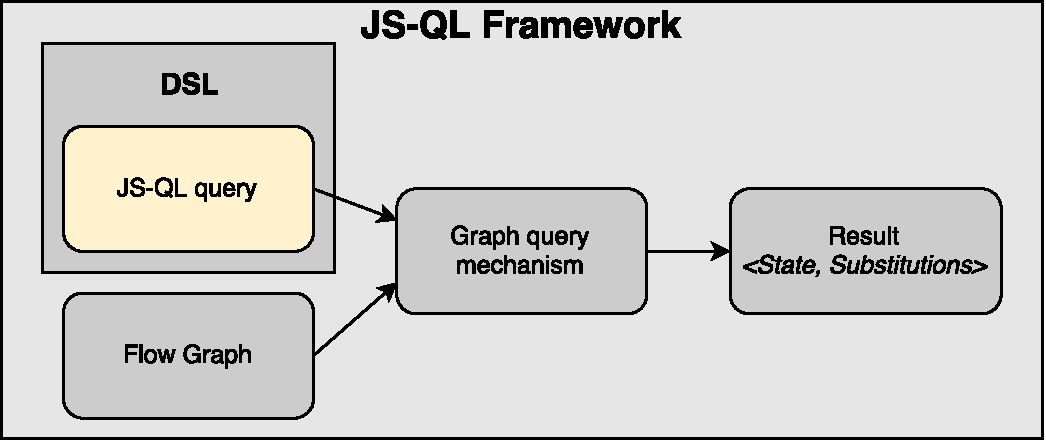
\includegraphics[width=0.9\textwidth]{images/Architecture} 
      \caption{JS-QL framework architecture}
    \label{fig:architecture}
\end{figure}
\section{Flow graphs for JavaScript programs}

The need for detailed control- and data flow information in our program representation graph limits the types of graphs that can be used for our framework. Program dependence graphs\cite{PDG} for example can be very useful to track the flow of information between certain points in a program but often lack more general information about program states, making them less qualified to use as our main program representation. In contrast, the JIPDA\cite{} abstract state graph contains all the information needed to precisely express patterns to be detected in a program. This section takes an in-depth look at the JIPDA abstract state graph and the information it holds in its states. Figure \ref{fig:JipdaGraph} shows part of a typical graph produced by JIPDA for a program containing a check for whether a number is equal to zero or not.

The abstract state graph can contain four different types of states. JIPDA internally uses Esprima\cite{Esprima} to parse JavaScript code and set up an abstract syntax tree (AST). This AST is the starting point for the analysis that JIPDA performs, hence information about the nodes from the AST is also contained in certain states in the resulting graph. These states are  marked in red and are so-called \textit{evaluation states}. 


\begin{figure}
    \centering
      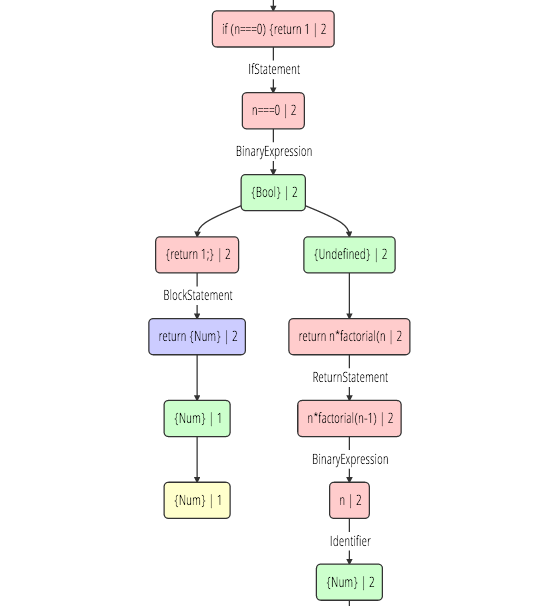
\includegraphics[width=262px, height=606px, keepaspectratio]{images/JipdaGraph} 
      \caption{Example JIPDA abstract state graph}
    \label{fig:JipdaGraph}
\end{figure}

%A control flow graph (CFG) in computer science is a representation, using graph notation, of all paths that might be traversed through a program during its execution.
%Jipda: abstract state graph containing information about control & data flow.
\section{Internal and external DSLs for querying graphs}
%https://msdn.microsoft.com/en-us/magazine/ee291514.aspx
%but the mechanics of creating an internal DSL are simpler because you are not employing compilers or parsers external to your code.
%Internal vs external
%DSL vs general purpose
\section{Design of an internal DSL for querying flow graphs}
%Flow graphs beperken predikaten, Extensibility, JavaScript, no REPL
%https://idl.cs.washington.edu/files/2014-Ellipsis-EuroVis.pdf --> Zij doen wel element van fluent API als argument -> Overwegen of gebruiken of niet


